\section{Übersicht Maschinentechnik}

\subsection{Beschreibung der Komponenten}

Die Konstruktion besteht hauptsächlich aus Aluminium-Blechteilen. Einige 
Komponenten müssen aus konstruktiven Gründen als Frästeile ausgeführt werden. 
Um ein geringeres Gewicht zu erreichen, werden die Blechteile mit Aussparungen 
an nicht erforderlichen Flächen versehen. Da dies eine Schwächung der 
Stabilität mit sich bringt, werden die Aussparungen, wie im Flugzeugbau 
üblich, mit gebogenen Innenkanten ausgeführt.

\begin{figure}[h!]
    \centering
    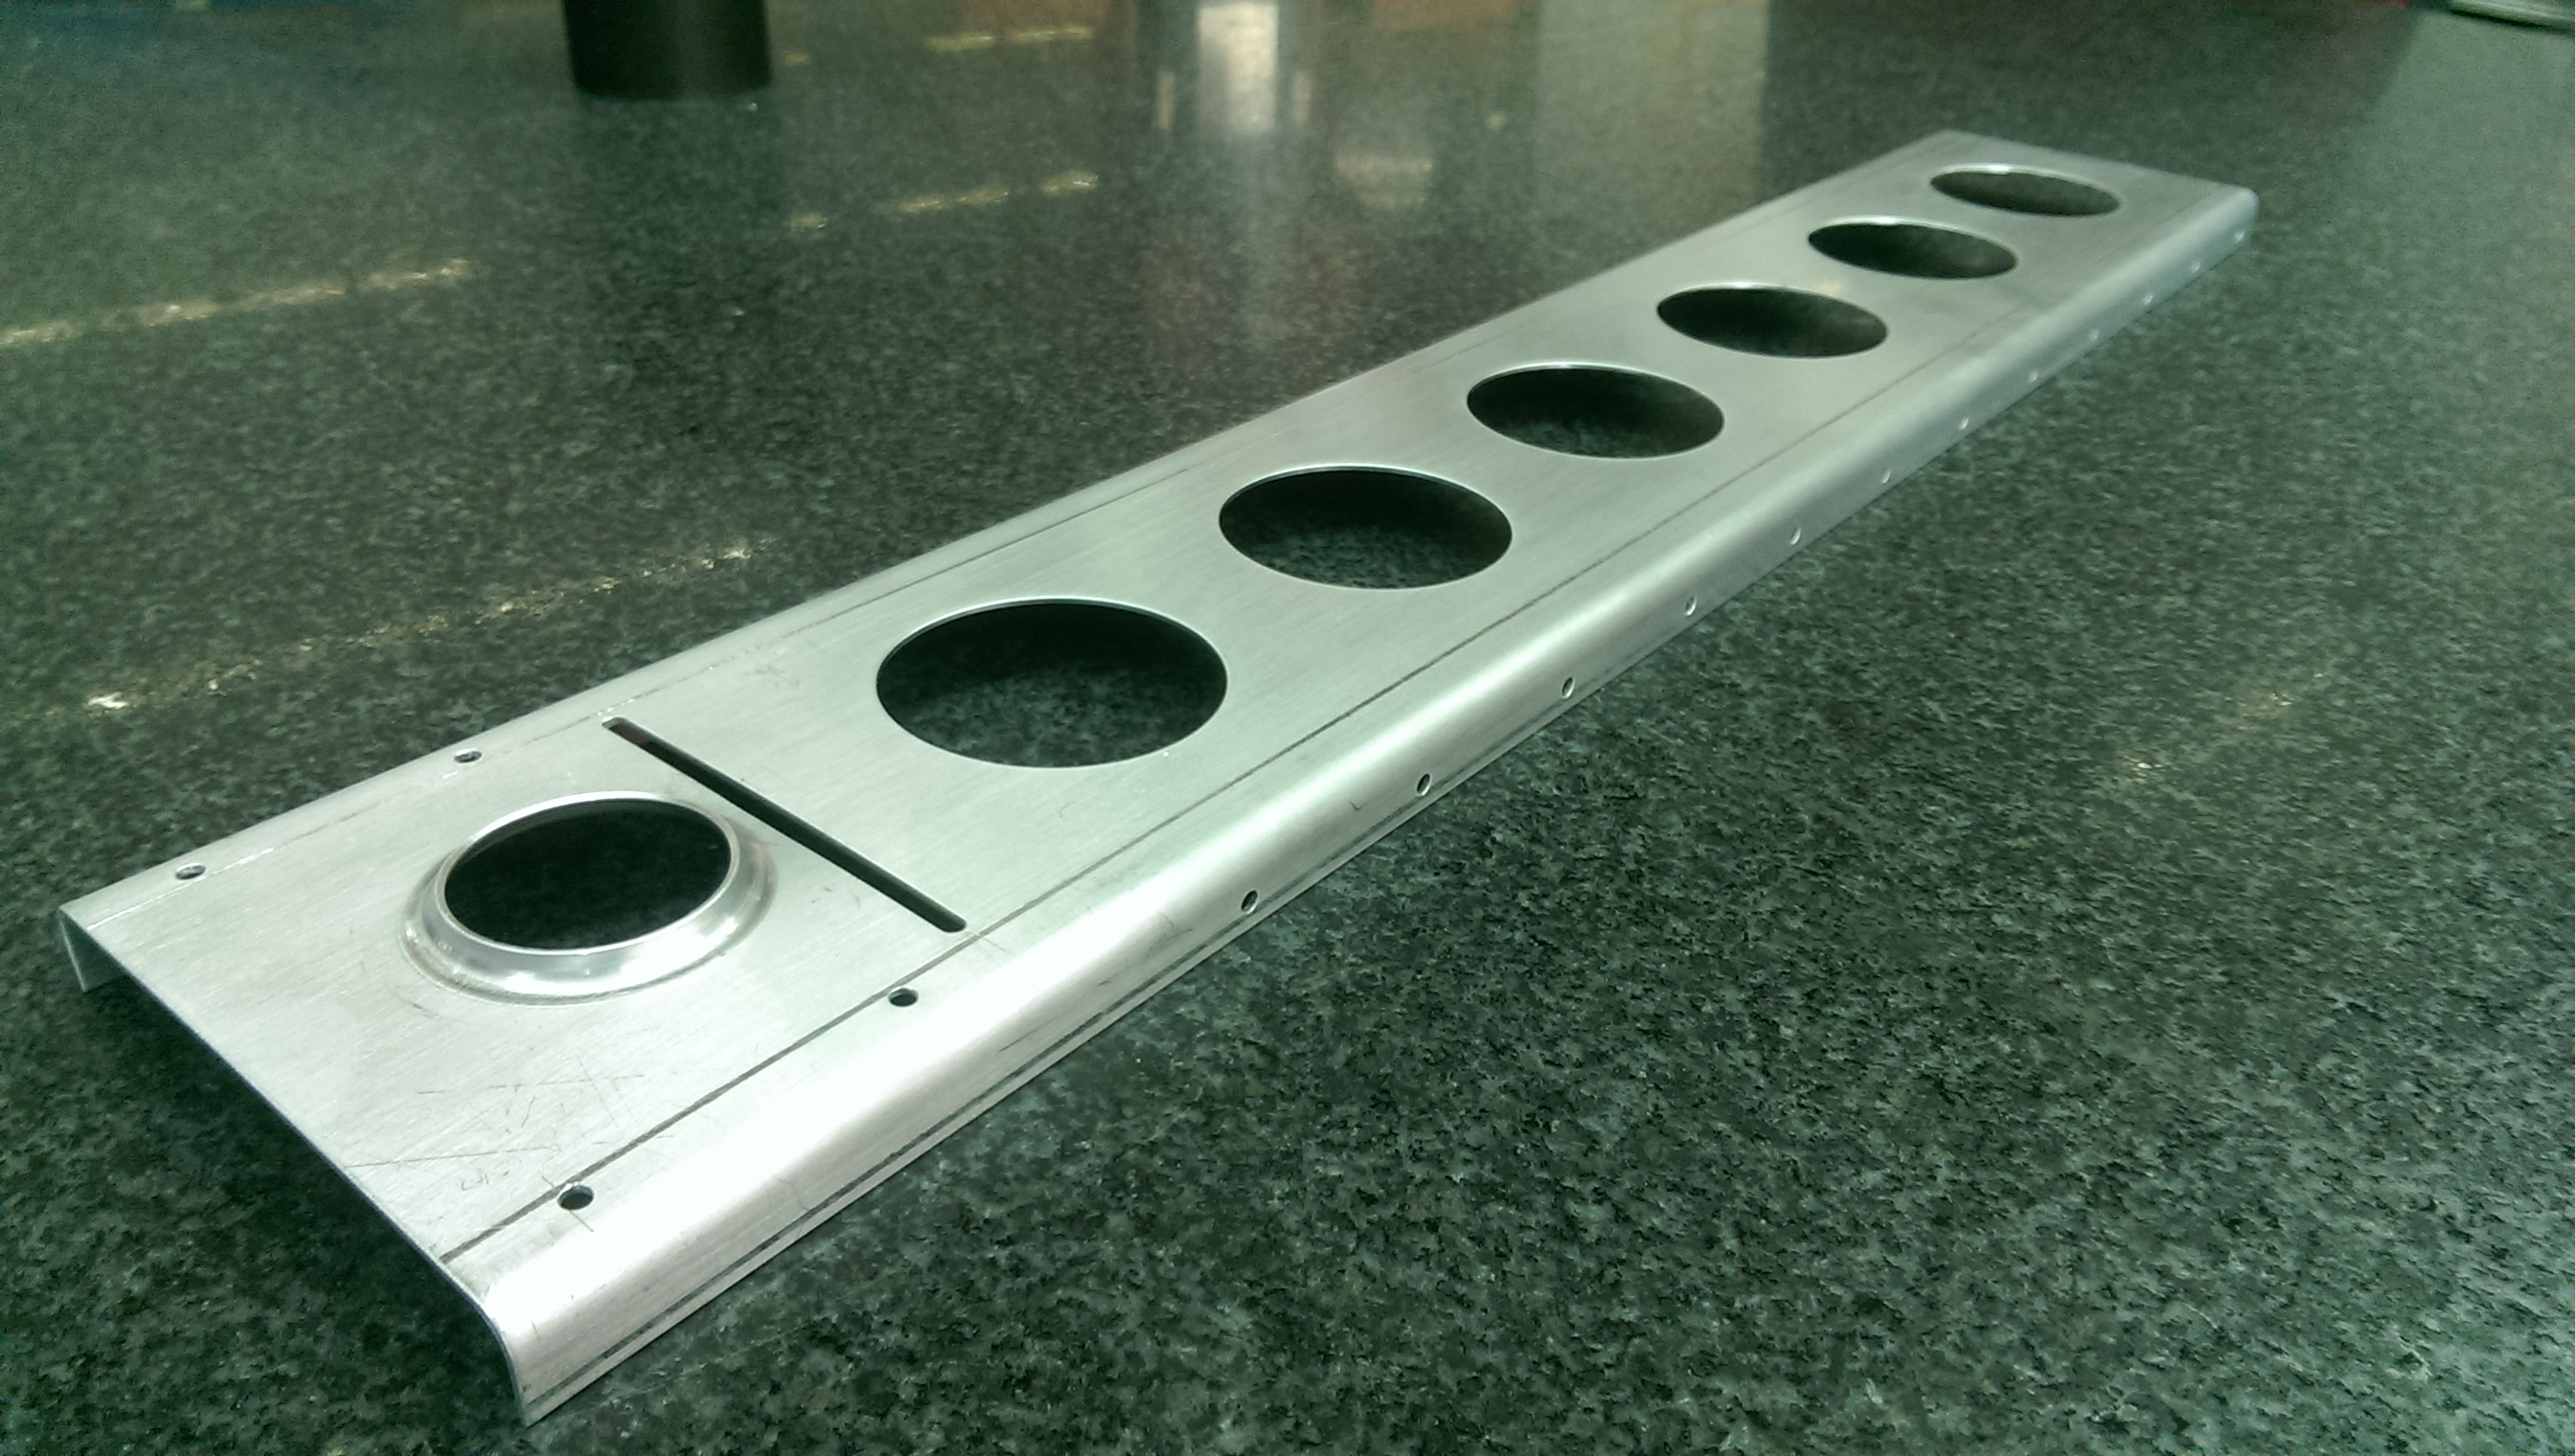
\includegraphics[width=0.5\textwidth]{fig/IMAG0364.jpg}
    \caption{Seitenteil Balllager}
    \label{fig:balllager_side}
\end{figure}

\subsubsection{Balllager}
Das Balllager dient als Grundstruktur, an welcher der Ballnachschub und der 
Motor befestigt sind. Gelagert werden die Bälle im Inneren des quadratischen 
Querschnittes. Die Halterungen des Motors werden jeweils auf beiden 
Aussenseiten des vorderen Endes befestigt. Damit das Stahlband des 
Ballnachschubs optimal aufgewickelt werden kann, werden die herausstehenden 
Enden der Nieten mit Aluminiumleisten abgedeckt. Diese können gleichzeitig als 
Kabelkanal verwendet werden. 

\begin{figure}[h!]
    \centering
    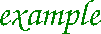
\includegraphics[width=0.5\textwidth]{../example/fig/example.pdf}
    \caption{Balllager}
    \label{fig:balllager}
\end{figure}

\subsubsection{Ballnachschub}
Der Ballnachschub besteht im Wesentlichen aus einer Trommel, einem Stahlband 
und einem Servomotor. Das Stahlband wird im Inneren des Balllagers um die 
Bälle herum ausgelegt. Durch das Aufwickeln des Bandes auf die Trommel werden 
die Bälle Richtung Beschleunigungsrad befördert. Der Antrieb erfolgt durch einen 
umgebauten Servomotor, welcher mittels Zahnriemen mit der Welle der Trommel 
verbunden ist.

\begin{figure}[h!]
    \centering
    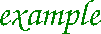
\includegraphics[width=0.5\textwidth]{../example/fig/example.pdf}
    \caption{Ballnachschub}
    \label{fig:ballnachschub}
\end{figure}

\paragraph{Auslegung}
Als Servo dient ein HS85MG der Firma Hitec. Dieses ist wie folgt spezifiziert: 
\begin{table}[h!]
    \centering
    \begin{zebratabular}{lll}
        \rowcolor{gray}
        Parameter &
        Wert bei 4.8\si{\volt} &
        Wert bei 6.0\si{\volt} \\
        Stellgeschwindigkeit (60\si{\degree}) &
        0.16\si{\second} &
        0.14\si{\second} \\
        Drehmoment &
        3.0\si{\kilogram\per\centi\metre} &
        3.5\si{\kilogram\per\centi\metre} \\
    \end{zebratabular}
    \caption{Spezifikation Servomotor Hitec HS85MG}
\end{table}
Dies ergibt folgende Spezifikationen für den sich daraus ergebenden DC Motor: 
\begin{table}[h!]
    \centering
    \begin{zebratabular}{lll}
        \rowcolor{gray}
        Parameter &
        Wert bei 4.8\si{\volt} &
        Wert bei 6.0\si{\volt} \\
        Drehzahl &
        62.5\si{\per\minute} &
        71.4\si{\per\minute} \\
        Drehmoment &
        0.3\si{\newton\metre} &
        0.35\si{\newton\metre} \\
    \end{zebratabular}
    \caption{Spezifikation DC Motor basierend auf Hitec HS85MG}
\end{table}
Beim Dauerbetrieb zeigt sich dieser Motor als zu schwach. Um eine akzeptable 
Abschusskadenz zu erreichen muss er mit einer Spannung von 16\si{\volt} 
betrieben werden. Dieser Belastung ist der Motor nicht gewachsen. Nach einigen 
Versuchen weist er einen Kurzschluss auf und muss ersetzt werden. Als Ersatz 
kommt ein Servo vom Typ TS-301 MGBB von Conrad zum Einsatz. Dieser kann an 
einer Spannung von 12\si{\volt} bei einem Tastgrad von 85\% problemlos 
betrieben werden. Gleichzeitig wird die Übersetzung des Riemenantriebs auf ein 
Verhältnis von 2:1 erhöht. 
\begin{table}[h!]
    \centering
    \begin{zebratabular}{ll}
        \rowcolor{gray}
        Parameter &
        Wert bei 4.8\si{\volt} \\
        Stellgeschwindigkeit (50\si{\degree}) &
        0.22\si{\second} \\
        Drehmoment &
        3.5\si{\kilogram\per\centi\metre} \\
    \end{zebratabular}
    \caption{Spezifikation Servomotor Conrad TS-301 MGBB}
\end{table}
Dies ergibt folgende Spezifikationen für den sich daraus ergebenden DC Motor: 
\begin{table}[h!]
    \centering
    \begin{zebratabular}{lll}
        \rowcolor{gray}
        Parameter &
        Wert bei 4.8\si{\volt} \\
        Drehzahl &
        37.9\si{\per\minute} \\
        Drehmoment &
        0.35\si{\newton\metre} \\
    \end{zebratabular}
    \caption{Spezifikation DC Motor basierend auf Conrad TS-301 MGBB}
\end{table}

\subsubsection{Drehvorrichtung}
Die Drehvorrichtung dient zur horizontalen Ausrichtung der 
Abschussvorrichtung. Um eine genaue Positionierung und ausreichende Stabilität 
zu ermöglichen, wird ein Zahnrad durch zwei Axial-Rillenkugellager auf einer 
Grundplatte verspannt. Die Ausrichtung wird durch einen Schrittmotor mit dem 
direkt verbundenen, kleineren Zahnrad realisiert. Einen guten Bodenkontakt 
garantieren an der Unterseite der Füsse angeklebte Gummimatten.

\begin{figure}[h!]
    \centering
    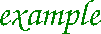
\includegraphics[width=0.5\textwidth]{../example/fig/example.pdf}
    \caption{Drehvorrichtung}
    \label{fig:drehvorrichtung}
\end{figure}

\paragraph{Auflösung}
Der Schrittmotor benötigt 200 Schritte für eine Umdrehung. Er wird mit 1/128 
Mikrosteps angesteuert. Die Übersetzung beträgt 1:4.8. Daraus ergibt sich 
folgende Auflösung: 
\[ 200 \cdot 128 \cdot 4.8 = 122'880 \frac{\text{Schritte}}{\text{Umdrehung}}  \]
\[ \frac{360^\circ}{122'880} = 0.0029296875 \frac{^\circ}{\text{Schritt}} 
= 0.17578 \frac{'}{\text{Schritt}} = 10.547 \frac{''}{\text{Schritt}}
\rightarrow 341.33 \frac{\text{Schritte}}{^\circ}\]

\subsubsection{Motor}
Der Motor für die Ballbeschleunigung wird als Eigenkonstruktion ausgeführt.  
Der Läufer dient dabei als Felge des Beschleunigungsrades und wird aus 
Aluminium gefräst. Als Grundlage für den Motor dienen Motoren aus 
Diskettenlaufwerken. Diese besitzen 10 Polpaare und 15 Nuten. Diese 
Konfiguration wird grundsätzlich beibehalten. Jedoch wird der neue Motor aus 
den Statorblechen von zwei Diskettenlaufwerkmotoren aufgebaut. Dies dient 
dazu, den magnetischen Querschnitt zu vergrössern. Für die Dauermagnete des 
Rotors kam im Laufwerk ein Magnetring zum Einsatz. Im neuen Rotor werden die 
Dauermagnete mittels Neodymmagneten realisiert. Dabei wird ein Halbach-Array 
aufgebaut. Deshalb kommen Magnete mit einer quadratischen Grundfläche zum 
Einsatz. 
\begin{figure}[h!]
    \centering
    
\includegraphics[width=0.5\textwidth]{fig/halbach.pdf}
    \caption{Ausschnitt aus verwendetem Halbach-Array mit Rückschlussring}
    \label{fig:halbach}
\end{figure}
Ein Halbach-Array hat den Vorteil, dass die Feldlinien auf einer 
Seite gebündelt werden, sich auf der Anderen hingegen beinahe aufheben. 
Als Rückschluss kommt ein Stahlring zum Einsatz, welcher in den Rotor 
eingepresst wird. Dieser dient dazu, die Magnetfeldlinien hinter den 
Dauermagneten zu bündeln und so den magnetischen Kreis zu schliessen. 

\begin{figure}[h!]
    \centering
    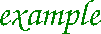
\includegraphics[width=0.5\textwidth]{../example/fig/example.pdf}
    \caption{Motor}
    \label{fig:motor}
\end{figure}

\subsubsection{Turm}
Der Turm dient als Verbindungselement des Balllagers mit dem grossen Zahnrad 
der Drehvorrichtung. Aufgebaut wird die gesamte Konstruktion aus 
Aluminiumblech. Der Platz im Inneren wird zum Verstauen der 
Elektronikkomponenten verwendet. Deswegen wird die vordere Abdeckplatte als 
Wartungsklappe ausgeführt. Die Abdeckplatte wird mit Schrauben anstatt mit 
Nieten befestigt.

\begin{figure}[h!]
    \centering
    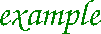
\includegraphics[width=0.5\textwidth]{../example/fig/example.pdf}
    \caption{Turm}
    \label{fig:turm}
\end{figure}
